%%%%%%%%%%%%%%%%%%%%%%%%%%%%%%%%%%%%%%%%%%%%%%%%%%%%%%%%%
%Este documento representa la plantilla de los articulos%
%a ser editados para la revista, realizada bajo codigo  %
%        Latex, con una clase ``article``               %   
%          PUBLICACIONES EN CIENCIAS                    %               
%                Y  TECNOLOGIA.                         %
%        Realizado por Adriana Araujo                   %
%       Revisado por Hugo Lara              (2014)      %        
%              Cuerpo editorial.                        %
%%%%%%%%%%%%%%%%%%%%%%%%%%%%%%%%%%%%%%%%%%%%%%%%%%%%%%%%%
\documentclass[11pt,twoside,A5]{article}
\usepackage[spanish]{babel}
\usepackage[utf8]{inputenc}
\usepackage{amsmath}
\usepackage{amsfonts}
\usepackage{amssymb}
\usepackage{amscd}
\usepackage{psfrag}
\usepackage{graphicx}
\usepackage{url}
%%%%%%%%%%%%%%%%%%%%%%%%%%%%%%%%%%
%\theoremstyle{theorem}
\newtheorem{thm}{Theorem}[section]
\newtheorem{prop}{Proposition}[section]
\newtheorem{clly}{Corollary}[section]
\newtheorem{lem}{Lemma}[section]
\newtheorem{pf}{Proof}[section]
%\theoremstyle{definition}
\newtheorem{defi}{Definition}[section]
\newtheorem{exam}{Example}[section]
\newtheorem{rk}{Remark}[section]
\def\proof{\mbox {\it Proof.~}}
\newcommand{\en}{\~n}
\newcommand{\figura}{\stepcounter{figure}}
\newcommand{\cuadro}{\stepcounter{table}}
\renewcommand{\tablename}{Tabla}
\newtheorem{pot}{Proof of Theorem} %\ref{mainthm}}
%%%%%%%%%%%%%%%%%%%%%%%%%%%%%%%%%%%%%%%%%%
\def\N{\mathbb{N}}
\def\Z{\mathbb{Z}}
\def\Q{\mathbb{Q}}
\def\R{\mathbb{R}}
\def\C{\mathbb{C}}
\def\K{\mathbb{K}}
\def\V{\mathbb{V}}
\def\U{\mathbb{U}}
\def\O{\mathcal{O}}
\def\A{\mathcal{A}}
\def\L{\mathcal{L}}
\def\Rc{\mathcal{R}}
\newcommand{\vect}{\overrightarrow}
\newcommand{\modN}{\;\text{(mod $N$)}}

\usepackage[pass,paperwidth=15cm,paperheight=22cm]{geometry}
\paperheight=22cm
  \paperwidth=15cm
\setlength{\oddsidemargin}{-0.5cm} \setlength{\evensidemargin}{-1.0cm}
\setlength{\topmargin}{-1.5cm} \setlength{\textwidth}{11.5cm}
\setlength{\textheight}{17.5cm}


\setcounter{page}{1}
%%%%%%%%%%%%%%%%%%%%%%%%%%%%%%%%%%

%%%%%%%%%%%%%%%%%%%%%%%%%%%%%%%%%%%%%%%
\usepackage{fancyhdr}
\pagestyle{fancy}
%%%%%%%%%%%%%%%%%%%%%%%%%%%%%%%%%%%%%%%%%%%%%%%%%%%%%%%%%%%%%%%%%%%%%%%%%%%%%%%%%%%%%%%%%%%%%%%%%%%%%%%%%%%%%%%
%%%%%%%%SECCION DEL TITULO Y TIRILLA BIBLIOGRAFICA(ESTA ULTIMA PARA USO INTERNO DEL CUERPO EDITORIAL)%%%%%%%%%%
%%%%%%%%%%%%%%%%%%%%%%%%%%%%%%%%%%%%%%%%%%%%%%%%%%%%%%%%%%%%%%%%%%%%%%%%%%%%%%%%%%%%%%%%%%%%%%%%%%%%%%%%%%%%%%%
\begin{document}
\title{
\vspace{-1.1in}
\begin{flushleft}
{\normalsize \begin{center}
%{\em\bf Publicaciones en Ciencias y Tecnolog\'ia}\\ 
%\scriptsize{Vol 7, N$^{0}$2, Jul--Dic 2013, pp.7--15,   ISSN:1856-8890, Dep\'osito Legal:pp200702LA2730 }
%\small{Art\'iculo en revisi\'on.  ISSN:1856-8890, Dep\'osito Legal: pp200702LA2730}
\end{center}}
\end{flushleft}
\hrule \vspace{0.5in}{ARQUITECTURA HÍBRIDA DE NAVEGACIÓN PARA ROBOT PIONEER PD3X} }
%%%%%%%%%%%%%%%%%%%%%%%%%%%%%%%%%%%%%%%%%%%%%%%%%%%%%%%%%%%%%%%%%%%%%%%%%%%%%%%%%%%%%%%%%%%%%%%%%%%%%%%%%%%%%%%
%%%%%%%%SECCION AUTORES Y FILIACION DE LOS MISMOS %%%%%%%%%%%%%%%%%%%%%%%%%%%%%%%%%%%%%%%%%%%%%%%%%%%%%%%%%%%%%%
%%%%%%%%%%%%%%%%%%%%%%%%%%%%%%%%%%%%%%%%%%%%%%%%%%%%%%%%%%%%%%%%%%%%%%%%%%%%%%%%%%%%%%%%%%%%%%%%%%%%%%%%%%%%%%%

\author{ 
\footnote{  {\it\scriptsize  Decanato de Ciencias y Tecnolog\'ia,} 
{\it\scriptsize Universidad Centroccidental Lisandro Alvarado,}
{\it\scriptsize Barquisimeto, Venezuela, sauljabin@gmail.com}
}\hspace{1mm}{Saúl Piña}
 \hspace{3mm} 
\footnote{  {\it\scriptsize  Decanato de Ciencias y Tecnolog\'ia,} 
{\it\scriptsize Universidad Centroccidental Lisandro Alvarado,}
{\it\scriptsize Barquisimeto, Venezuela, thejorgemylio@gmail.com}
}\hspace{1mm}{ Jorge Parra} \\
 %\hspace{3mm} 
%\footnote{  {\it\scriptsize Departamento-Instituto-Facultad}, 
%{\it\scriptsize Universidad-Instituci\'on (filiaci\'on)},
%{\it\scriptsize Lugar, Pa\'is, email}
%}\hspace{5mm}{ Nombre autor 3 }
% \hspace{3mm} 
%\hspace{3mm}
%\footnote{ {\it\scriptsize  Departamento de Ingenier\'ia Industrial,  Instituto Tecnol\'ogico de Celaya}, 
%{\it\scriptsize Instituto Tecnol\'ogico de Celaya},  
%{\it\scriptsize M\'exico, gesparza@itc.mx }
%}\hspace{5mm} { Luis Gerardo Esparza-D\'iaz}
}

%\vspace{-15mm}
\date{\small{Octubre 2014}
}

%\date{}
%%%%%%%%%%%%%%%%%%%%%%%%%%%%%%%%%%
\maketitle 
%%%%%%%%%%%%%%%%%%%%%%%%%%%%%%%%%%%%%%%%%%%%%%%%%%%%%%%%%%%%%%%%%%%%%%%%%%
% SECCION TITULO CORTO E INICIALES AUTORES, HASTA DOS AUTORES:
% APELLIDO 1, INICIAL NOMBRE 1. ; APELLIDO 2, INICIAL NOMBRE 2.
%                        MAS DE DOS 
%                APELLIDO, INICIAL NOMBRE. et al
%%%%%%%%%%%%%%%%%%%%%%%%%%%%%%%%%%%%%%%%%%%%%%%%%%%%%%%%%%%%%%%%%%%%%%%%%%%
\fancyhead{} \fancyhead[CE]{ ARQUITECTURA HÍBRIDA DE NAVEGACIÓN PARA ROBOT PIONEER PD3X  }
\fancyhead[CO]{ Saúl Piña, Jorge Parra 
}
\fancyfoot{}
%\fancyfoot[CO,CE]{\scriptsize{{Publicaciones en Ciencias y Tecnolog\'ia.} Vol 7,N$^{0}$2, Jul--Dic 2013, pp.07--15.}}
%\fancyfoot[CO,CE]{Publicaciones en Ciencias y Tecnolog\'ia. Art\'iculo en revisi\'on}
\fancyfoot[RO,LE]{\thepage}

%%%%%%%%%%%%%%%%%%%%%%%%%%%%%%%%%%%%%%%%%%%%%%%%%%%%%%%%%%%%%%%%%%%%%%%%%%%%%
%%%%%%%%%%%%%%%%%%SECCION DE RESUMEN Y ABSTRACT%%%%%%%%%%%%%%%%%%%%%%%%%%%%%%
%%%%%%%%%%%%%%%%%%%%%%%%%%%%%%%%%%%%%%%%%%%%%%%%%%%%%%%%%%%%%%%%%%%%%%%%%%%%%
\begin{center}
{\bf\small Resumen}
%\vspace{-5mm}

\vspace{-3mm} \hspace{.05in}\parbox{4.5in} {{\small %\footnotesize 



 \textbf{Palabras clave}: Robótica, ARIA, AuRA, Arquitectura Híbrida, Pioneer P3DX}}
\end{center}
\pagebreak


%\begin{center}
%{\bf\small T\'ITULO EN INGL\'ES \\ Abstract}
%
%\vspace{-3mm} \hspace{.05in}\parbox{4.5in} {{\small %\footnotesize 
%
%Cuerpo del abstract  
%
%     \textbf{Keywords}:  kw 1, kw 2, ... .}}
%\end{center}
%%%%%%%%%%%%%%%%%%%%%%%%%%%%%%%%%%%%%%%%%%%%%%%%%%%%%%%%%%%%%%%%%%%%%%%%%%%%%%%%%%%%%%%
%                           CUERPO DEL ARTICULO
%%%%%%%%%%%%%%%%%%%%%%%%%%%%%%%%%%%%%%%%%%%%%%%%%%%%%%%%%%%%%%%%%%%%%%%%%%%%%%%%%%%%%%%
%\pagebreak

\section*{Introducción}

\section*{Pioneer P3DX}

\begin{figure}[here]
\begin{center}
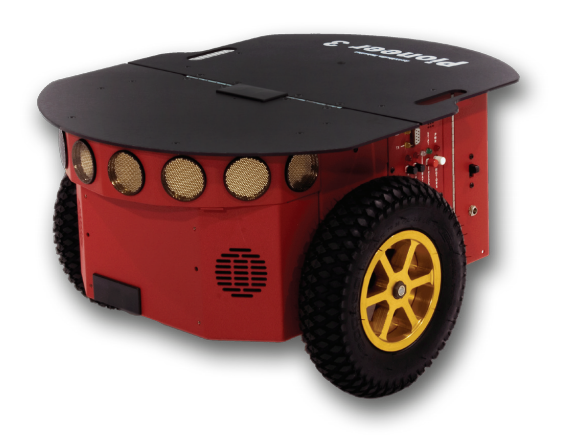
\includegraphics[width=6cm]{pioneer.png} 
\caption{Robot Pioneer P3DX}
\label{fig:pioneer}
\end{center}
\end{figure} 

\section*{Arquitectura AuRA}


\section*{Implementación de la Arquitectura}


\section*{Entorno de Desarrollo}

Para llevar a cabo la presente investigación se desarrollo una aplicación cliente
con las siguientes herramientas de software:

\textbf{ARIA} (Advanced Robot Interface for Applications) \cite{aria2014},
es una librería desarrollada en el lenguaje de programación C++ para todas las
plataformas MobileRobots/ActivMedia. Provee el conjunto de herramientas necesarias
para controlar y monitorear de forma dinámica al robot y sus elementos. Ademas, esta librería
incluye implementaciones llamadas \textit{wrapper} en los lenguajes de programación Python y Java, siendo este último 
el lenguaje de desarrollo para este investigación.

\textbf{MobileSim} \cite{mobilesim2014}, es un software para la simulación de plataformas
MobileRobots/ActivMedia. Permite usar la librería ARIA y sus wrappers. Es un ambiente
ideal para realizar experimentación y pruebas de los algoritmos desarrollados antes de
implementarlos en los robots reales.
 
\textbf{Eclipse IDE} \cite{eclipse2014}, es un entorno de desarrollo integrado para múltiples lenguajes de 
programación en los que destacan Java y C++. Provee de las herramientas necesarias para el desarrollo, depuración  
y compilación de aplicaciones.

\textbf{Java} \cite{java2014}, es un lenguaje de programación de propósito general, orientado a objetos y de alto nivel. 
 
\section*{Configuración del Entorno}

Antes de configurar el entorno de desarrollo es necesario descargar el código fuente del proyecto,
este está disponible al público con licencia de software \textit{GPL} en la siguiente dirección:
\\ \url{https://bitbucket.org/sauljabin/ariajava-p3dx}.

\subsubsection*{\textit{Configuración del Entorno Sobre Windows}}

\begin{enumerate}
\item Previamente instalar Java y Eclipse.
\item Instalar \textbf{MobileSim-0.7.2-1.exe}. Disponible en: \\ \url{http://robots.mobilerobots.com/wiki/MobileSim}.
\item Instalar \textbf{ARIA-2.7.6.exe}. Disponible en: \\ \url{http://robots.mobilerobots.com/wiki/ARIA}.
\item Agregar a las variables de entorno del sistema la ruta \\ \url{C:\Program Files\MobileRobots\ARIA\bin\}.
\item Dirigirse a la ruta \url{C:\Program Files\MobileRobots\ARIA\bin\}, cambiar el nombre del archivo
	  \textbf{AriaVC10.dll} a \textbf{Aria.dll}.
\item Importar proyecto en eclipse.
\item Verificar que la variable \textbf{PATH\_LIBARIA} \\ del archivo \textbf{CONFIG.properties} 
	  sea igual a: \\ \url{C\:\\Program Files\\MobileRobots\\ARIA\\bin\\}
\end{enumerate}

\subsubsection*{\textit{Configuración del Entorno Sobre Debian/Ubuntu}}

\begin{enumerate}
\item Previamente instalar Java y Eclipse. 
\item Descargar el archivo \textbf{MobileSim-0.7.3+gcc4.6.tgz}. Disponible en: \\ \url{http://robots.mobilerobots.com/wiki/MobileSim}.
\item Ejecutar los siguientes comandos por consola para instalar MobileSim:
{\ttfamily \footnotesize 
\\ \$ tar xzvf MobileSim-0.7.3+gcc4.6.tgz
\\ \# mv -f MobileSim-0.7.3 /usr/local/MobileSim
\\ \# ln -s -f /usr/local/MobileSim/MobileSim /usr/bin/mobilesim}
\item Descargar el archivo \textbf{ARIA-2.8.1+gcc4.6.tgz}. Disponible en: \\ \url{http://robots.mobilerobots.com/wiki/ARIA}.
\item Ejecutar los siguientes comandos por consola para instalar ARIA:
{\ttfamily \footnotesize 
\\ \$ tar xzvf ARIA-2.8.1+gcc4.6.tgz
\\ \# mv -f Aria-2.8.1 /usr/local/Aria
\\ \# echo '/usr/local/Aria/lib' > /etc/ld.so.conf.d/aria.conf
\\ \# ldconfig}
\item Importar proyecto en eclipse.
\item Verificar que la variable \textbf{PATH\_LIBARIA} \\ del archivo \textbf{CONFIG.properties} 
	  sea igual a: \\ \url{/usr/local/Aria/lib/}
\end{enumerate}

\section*{Herramienta de Software Desarrollada}


\section*{Experimentación}


%%%%%%%%%%%%%%%%%%%%%%%%%%%%%%%%%%%%%%%%%%%%%%%%%%%%%%%%%%%%%%%%%%%%%%%%%%%%%%%%%%%%%%%%
%                                 BIBLIOGRAFIA
%%%%%%%%%%%%%%%%%%%%%%%%%%%%%%%%%%%%%%%%%%%%%%%%%%%%%%%%%%%%%%%%%%%%%%%%%%%%%%%%%%%%%%%%
\begin{thebibliography}{999}

\bibitem{arkin1997}
	Arkin, R. y Balch, T. (1997).
 	AuRA: Principles and practice in review.
	Journal of Experimental \& Theoretical Artificial Intelligence.
	Taylor \& Francis. Vol. 9. No. 2-3. Pp. 175-189.
	
\bibitem{aria2014} 
	MobileRobots. (2014).
	ARIA. 	
	Disponible en: \url{http://robots.mobilerobots.com/wiki/ARIA}.
	
\bibitem{mobilesim2014} 
	MobileRobots. (2014).
	MobileSim. 	
	Disponible en: \url{http://robots.mobilerobots.com/wiki/MobileSim}.
	
\bibitem{eclipse2014} 
	Eclipse. (2014).
	Eclipse IDE. 	
	Disponible en: \url{https://www.eclipse.org/ide/}.

\bibitem{java2014} 
	Oracle. (2014).
	Java. 	
	Disponible en: \url{http://www.oracle.com/technetwork/java/index.html}.

\end{thebibliography}
\end{document}
